\documentclass[DIV=calc, paper=a4, fontsize=11pt, twocolumn]{scrartcl}	 % A4 paper and 11pt font size

\usepackage{lipsum} % Used for inserting dummy 'Lorem ipsum' text into the template
\usepackage[english]{babel} % English language/hyphenation
\usepackage[protrusion=true,expansion=true]{microtype} % Better typography
\usepackage{amsmath,amsfonts,amsthm} % Math packages
\usepackage[svgnames]{xcolor} % Enabling colors by their 'svgnames'
\usepackage[hang, small,labelfont=bf,up,textfont=it,up]{caption} % Custom captions under/above floats in tables or figures
\usepackage{booktabs} % Horizontal rules in tables
\usepackage{fix-cm}	 % Custom font sizes - used for the initial letter in the document
\usepackage{graphicx} % Package to insert images

\usepackage{sectsty} % Enables custom section titles
\allsectionsfont{\usefont{OT1}{phv}{b}{n}} % Change the font of all section commands

\usepackage{fancyhdr} % Needed to define custom headers/footers
\pagestyle{fancy} % Enables the custom headers/footers
\usepackage{lastpage} % Used to determine the number of pages in the document (for "Page X of Total")

% Headers - all currently empty
\lhead{COMSOL Lab 9}
\chead{}
\rhead{Spring 2024}

% Footers
%\lfoot{\footnotesize Instructor: } % Instructor's Name
%\cfoot{\footnotesize TA: } % TA's Name
\rfoot{\footnotesize Page \thepage\ of \pageref{LastPage}} % Format for Footnote: Page 1 of 2

\renewcommand{\headrulewidth}{0.0pt} % No header rule
\renewcommand{\footrulewidth}{0.4pt} % Thin footer rule

\usepackage{lettrine} % Package to accentuate the first letter of the text
\newcommand{\initial}[1]{ % Defines the command and style for the first letter
\lettrine[lines=3,lhang=0.3,nindent=0em]{
\color{DarkGoldenrod}
{\textsf{#1}}}{}}


%----------------------------------------------------------------------------------------
%	TITLE SECTION
%----------------------------------------------------------------------------------------

\usepackage{titling} % Allows custom title configuration

\newcommand{\HorRule}{\color{DarkGoldenrod} \rule{\linewidth}{1pt}} % Defines the gold horizontal rule around the title

\pretitle{\vspace{-30pt} \begin{flushleft} \HorRule \fontsize{30}{30} \usefont{OT1}{phv}{b}{n} \color{DarkRed} \selectfont} % Horizontal rule before the title

% Lab Report Title Goes Here
\title{Diffusion and Advection} 
% Lab Report Title Goes Here

\posttitle{\par\end{flushleft}\vskip 0.5em} % Whitespace under the title

\preauthor{\begin{flushleft}\large \lineskip 0.5em \usefont{OT1}{phv}{m}{sl} \color{Black}} % Author font configuration

% Student's name(s)
\author{Henry Arhin } 
% Student's name(s)

% Student's Institution
\postauthor{\footnotesize \lineskip 0.5em \usefont{OT1}{phv}{m}{sl} \color{Black} % Configuration for the institution name
 Clemson University\\ 
% Student's institution

\par\end{flushleft}\HorRule} % Horizontal rule after the title

\date{} % Add a date here if you would like one to appear underneath the title block

%----------------------------------------------------------------------------------------

\begin{document}

\maketitle % Print the title

\thispagestyle{empty} % Enabling the custom headers/footers for the second page forward

%----------------------------------------------------------------------------------------
%	ABSTRACT
%----------------------------------------------------------------------------------------

% The first character should be within \initial{}
\initial{T}\textbf{ransport problems in porous media can be modeled by diffusion and advection equations. Advection is simply transport of substances or quantities due to mass movement of fluids, and diffusion on the other hands is the movement of materials in porous media due to concentration gradient. In this lab, I will focused on these two physical phenomena and discuss the equations that model these modes of transport of substances.}

%----------------------------------------------------------------------------------------
%	ARTICLE CONTENTS
%----------------------------------------------------------------------------------------

\section*{Introduction}

Advection and diffusion are important processes which govern the transport of contaminant in a porous medium. These processes play a pivotal role in the knowing a particular remediation technique to apply to clean any field that has been contaminated by NAPL. These processes also play a very crucial role in geothermal heat evolution which informs the extraction of heat energy for power generation. The Peclet number relates the advection to the diffusion and is used to determine the width of plume. 

In this lab, the advection and diffusion of concentrated plume which has been injected into a fraction opening in a less permeable matrix was modeled to see how the concentrated source advects in the fracture and at the same time diffuses through the matrix as time evolves.
This lab will discuss the derivation of the general equation from the conservation of mass.

\begin{equation}
    \nabla \cdot (\Gamma + \frac{\partial c}{\partial t}) = s
\end{equation}

Where:
\begin{conditions}
  
\\c & : Concentration \\
\\t & : Time \\
\\s & : Source/Sink term
\end{conditions}


The symbol $\Gamma$ represents the summation of diffusion, which comprises the matrix diffusion described by Fick's law, hydrodynamic dispersion, and advection. The matrix diffusion typically represents the diffusion within a porous medium, and hydrodynamic dispersion refers to the spreading of a solute due to velocity variations within the fluid. Both are mechanisms contributing to the overall dispersion of solutes in a porous medium. The $\Gamma$ then is given by the equation:

\begin{equation}
\Gamma = A + D
\end{equation}

where $A$ represents advection and $D$ denotes the total diffusion.


%------------------------------------------------

\section*{Methodology}

The whole set-up was based on the first principles of diffusion and advection which was borne out of the laws of conservation. The model was created with two blocks and a fraction with an opening of 0.01m was created in between the two blocks. The advective flux is given as:
\begin{equation}
A = \mathbf{q} C
\end{equation}

Where:
\begin{conditions}
A & : Advective flux \
$\mathbf{q}$ & : Flow velocity vector \
c & : Concentration
\end{conditions}

The diffusive Fick's law is given by:

\begin{equation}
D = -D^* \nabla c
\end{equation}

Where:
\begin{conditions}
    $D$ & : Total diffusive flux \\
    $D^*$ & : Matrix diffusion coefficient \\
    $c$ & : Concentration
\end{conditions}

The dispersive flux is given by:

\begin{equation}
D_m = -D_m \nabla c
\end{equation}

Where:
\begin{conditions}
    $D_m$ & : Hydrodynamic dispersion coefficient \\
    $c$ & : Concentration
\end{conditions}

Therefore, the total diffusive flux \( D \) is given by the sum of the diffusive Fick's law and the dispersive flux:

\begin{equation}
D = D^* + D_m
\end{equation}

Where:
\begin{conditions}
    $D$ & : Total diffusive flux \\
    $D^*$ & : Matrix diffusion coefficient \\
    $D_m$ & : Hydrodynamic dispersion coefficient
\end{conditions}

These equations describe the transport of solutes in porous media, accounting for both diffusion and dispersion mechanisms.

\begin{equation}
\nabla \cdot (-(D^* + D_m)\nabla\cdot C ) + \nabla\cdot qC + \frac{\partial c}{\partial t} = s
\end{equation}

Set \( s \) to be 0:
\begin{equation}
\nabla \cdot (-(D^* + D_m)\nabla\cdot C) + \nabla\cdot qC + \frac{\partial c}{\partial t} = 0
\end{equation}

Rewriting it in a more compact form and assuming homogeneity as well as flux divergence free:

\begin{equation}
\frac{\partial C}{\partial t} = D \nabla^2 C - \mathbf{q} \cdot \nabla C
\end{equation}

Where:
\begin{conditions}
    \( c \) & : Concentration \\
    \( t \) & : Time \\
    \( \Gamma \) & : Total transport processes \\
    \( s \) & : Source/Sink term \\
    \( D \) & : Total diffusive flux \\
    \( \mathbf{q} \) & : Velocity vector \\
\end{conditions}



\subsection*{Boundary Conditions}

The boundary conditions used for the model were specified cncentration- Dirichlet boundary condition which the concentration for the lefthandside fracture was specified to be one.The model also had the flux which is normal to the surface which is the Neumann condition was specified for both the diffusive and advective fluxes.The hydraulic head on the right had side of the fracture was specified to be 0.




\section*{Results and Discussion}
\begin{figure}
  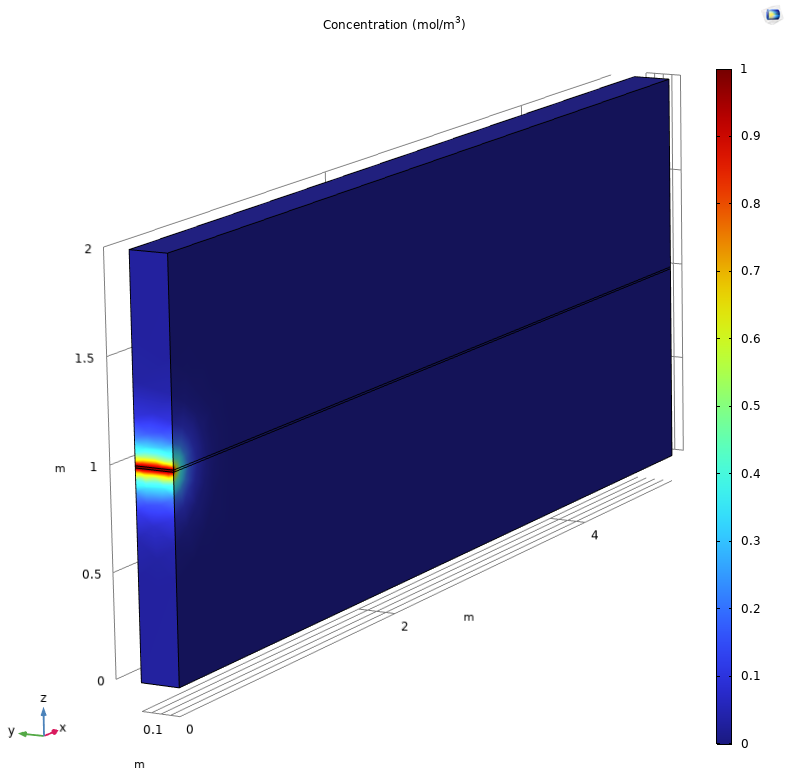
\includegraphics[width=\linewidth]{Concentration.png}
  \caption{Image of the evolution of concentration with time}
  \label{fig3}
\end{figure}
This model was supposed to model the diffusion of NAPL as it travels through a fracture in a matrix of less permeable medium. The NAPL concentration was supposed to have evolved with time and advected with the flowing water as well as diffuse in the matrix with time, but this phenomenon was not observed from the model. Adjustments need to be made to my model to adequately model this process.

%------------------------------------------------


\section*{Conclusion}
Coupling COMSOL with Matlab allows flexibility in the entire model; it particularly comes in handy when it comes to extracting useful information from the model for visualization and communication purposes.Since numerical models are supposed to compute a real world event, having adequate leverage over how the model is visualized is paramount. And this flexibility can be utilize in a great way when there is coupling between the COMSOL model and its codes in Matlab. Overall, I think I would like to work on the model further for a more meaningful extraction of information.


\end{document}
